\section{Diagramma delle classi}
\label{sec:diagramma delle classi}
Durante lo sviluppo della parte back-end, sono state create diverse classi per la gestione e interazione con il DataBase. 
\\ E' stata creata una classe principale contenente il metodo main, nella prima parte ci sono le inizializzazioni delle  componenti fondamentali, successivamente lancia il job di Spark.
\\ Come in figura \ref{fig:UMLSD}, sono state create classi contenitori a supporto dell'intera applicazione. 

\begin{figure}
	\centering
	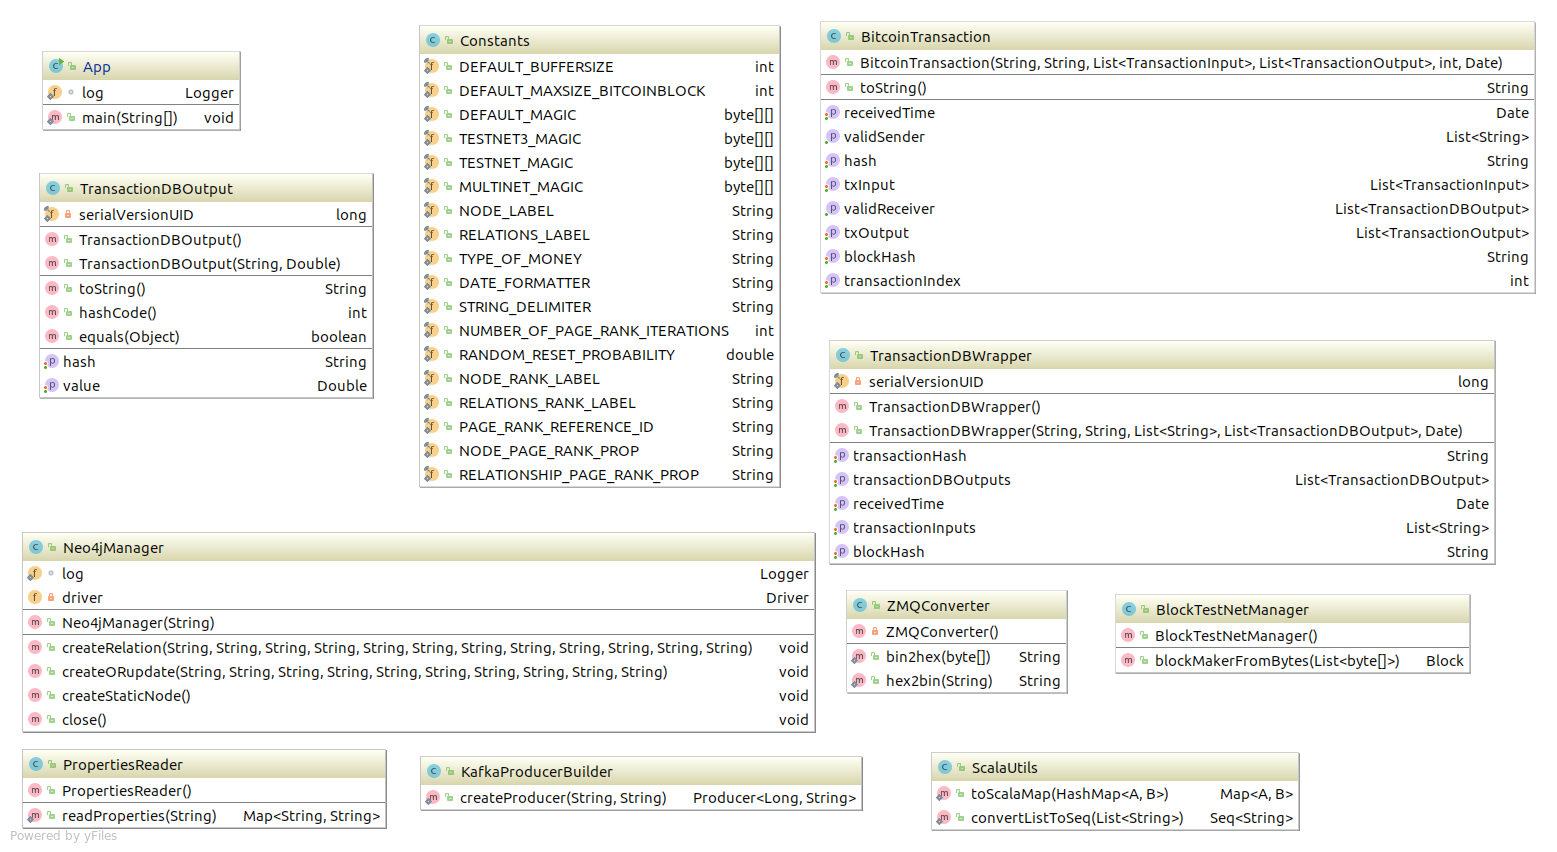
\includegraphics[width=\textwidth]{images/AppUML.png}
	\caption{UML delle classi (Sistema distribuito).}
	\label{fig:UMLSD}
\end{figure}
 
Per la parte front-end, ovvero la componente grafica dell'applicativo, 